\section{Dinâmica dos slides}
\label{sec:din}

Os slides podem ser tornados mais dinâmicos por meio de animações e transições. Uma animação ocorre dentro do slide, com os itens e imagens, já uma transição ocorre entre slides.

A princípio as transições devem ser usadas com muito cuidado, pois elas tem um impacto forte na atenção da audiência. Elas devem ser usadas apenas quando fazem sentido em relação ao fluxo ou ao conteúdo da apresentação. Considero que transições são praticamente proibidas em apresentações mais formais como defesas de tese.

Já as animações são um efeito muito útil, mas muitas vezes abusadas pelos apresentadores. Por exemplo, em uma lista de itens, como a da Figura \ref{fig:coppe}, alguns apresentadores poderiam escolher apresentar item a item e até mesmo tirar a cor dos itens já apresentados. Isto está errado, pois a platéia perde a visão global do assunto e a relação entre os itens a serem falados. Não devemos tratar a plateia como seres incapazes de separar um item do outro.

Os efeitos  básicos de ``aparecer'' ou ``desaparecer'', de várias formas, só devem ser usados para a construção de raciocínio. Um exemplo típico é o uso do efeito de aparecer quando uma fórmula está sendo derivada.

O efeito de ``aparecer'' é muito útil na solução de exercícios. Ele permite que os itens sejam mostrados passo a passo na apresentação, mas estejam todos no slide final, que pode ser impresso ou colocado em PDF. O slide da Figura \ref{fig:canvas} usa o efeito de aparecer para posicionar os \textit{post-its} em um canvas, um a um. Isso é feito durante a resolução de um exemplo. Todos os \textit{post-its} se mantém na imagem, como acontece no uso do canvas no mundo real. Nesse caso, porém, nem todos são totalmente legíveis, o que prejudica o uso final dos slides.


\begin{figure}[htb]
    \centering
    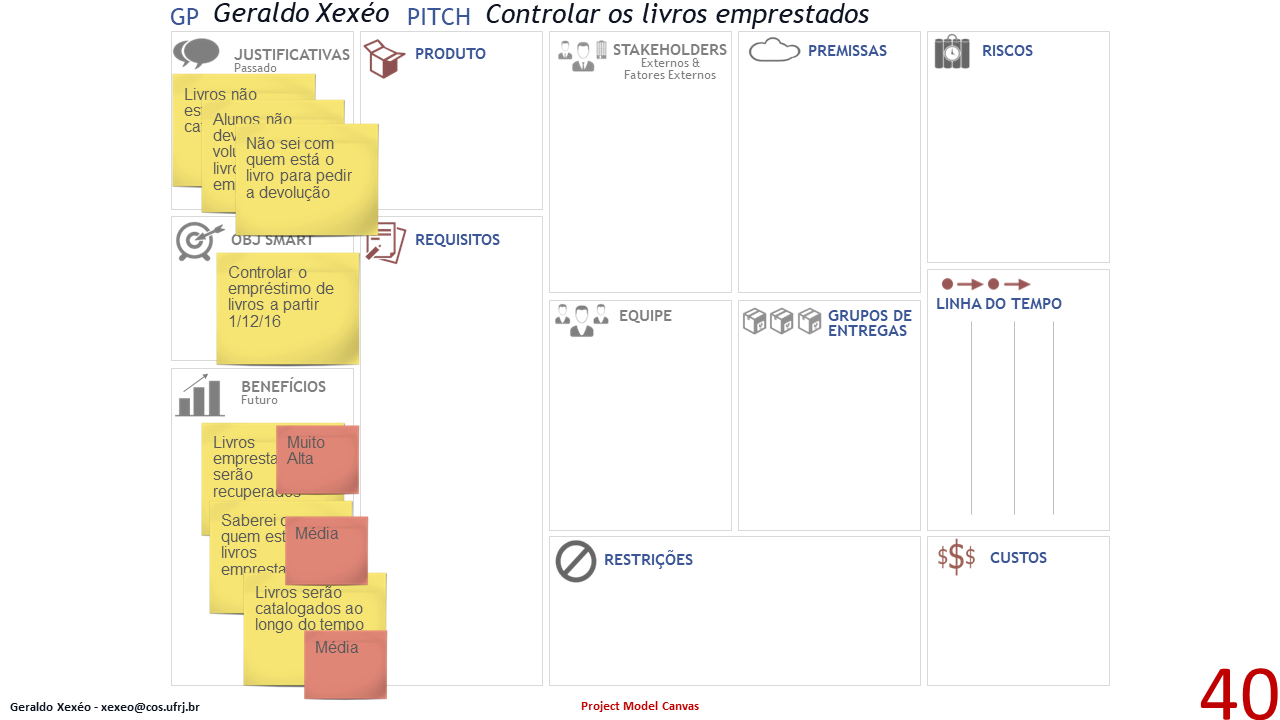
\includegraphics[width=0.7\linewidth,frame]{imagens/canvas}
    \caption{Esse slide usa o efeito de ``aparecer'' para mostrar os \textit{post-its} um a um.}
    \label{fig:canvas}
\end{figure}


O efeito de aparecer também pode ser simulado usando vários slides. Isso é uma estratégia essencial se os slides forem usados no formato PDF.


Aliás, o efeito de desaparecer deve ser usado com mais cuidado do que o de aparecer, já que a informação de que algo foi tirado do slide pode ser importante para entender o contexto global quando o slide é visto após a apresentação, ou quando alguém chega a apresentação no meio do slide. Em alguns casos é melhor usar o efeito de retirar a cor ou colocar alguma marca, como um X, sobre o que iria ser retirado do slide.

A Figura \ref{fig:passos} mostra dois passos em sequência de uma animação apresentada slide a slide enquanto o professor descreve como problemas de comunicação podem fazer um sistema não ser aceito pelos usuários. Todos os balões da primeira imagem vão aparecendo ao longo da narrativa, enquanto o professor fala e clica. Eles são mantidos na imagem para mostrar que as ideias e conversas continuam ao longo do projeto, além de facilitar o entendimento geral, e letras são usadas para quem olhar para dar alguma noção de ordem. Porém, quando o sistema é entregue, e as conversas ``param'', uma mudança ocorre e todos os balões são apagados. Este me parece um uso adequado do mecanismo de desaparecimento.

\begin{figure}[hbt]
    \centering
    \subfloat{
    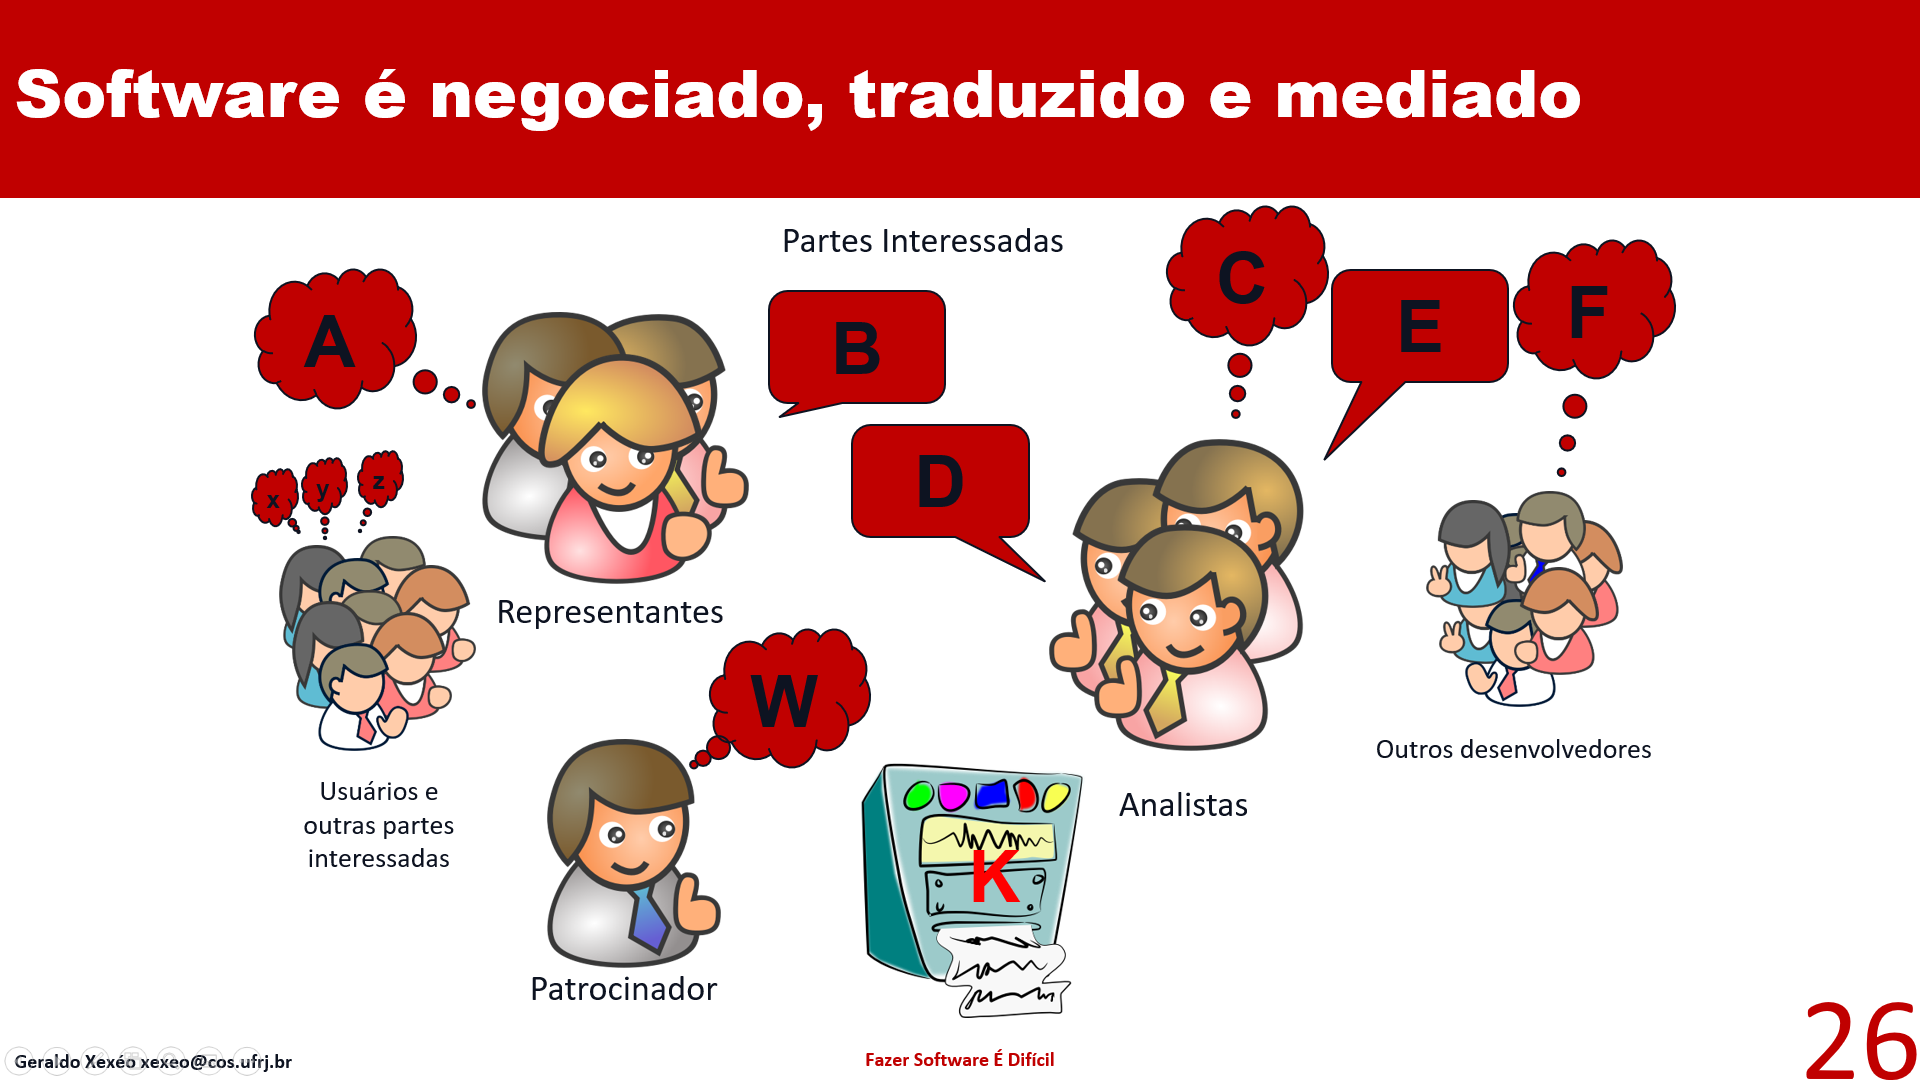
\includegraphics[width=0.4\linewidth,frame]{imagens/passo1}}
    \subfloat{
    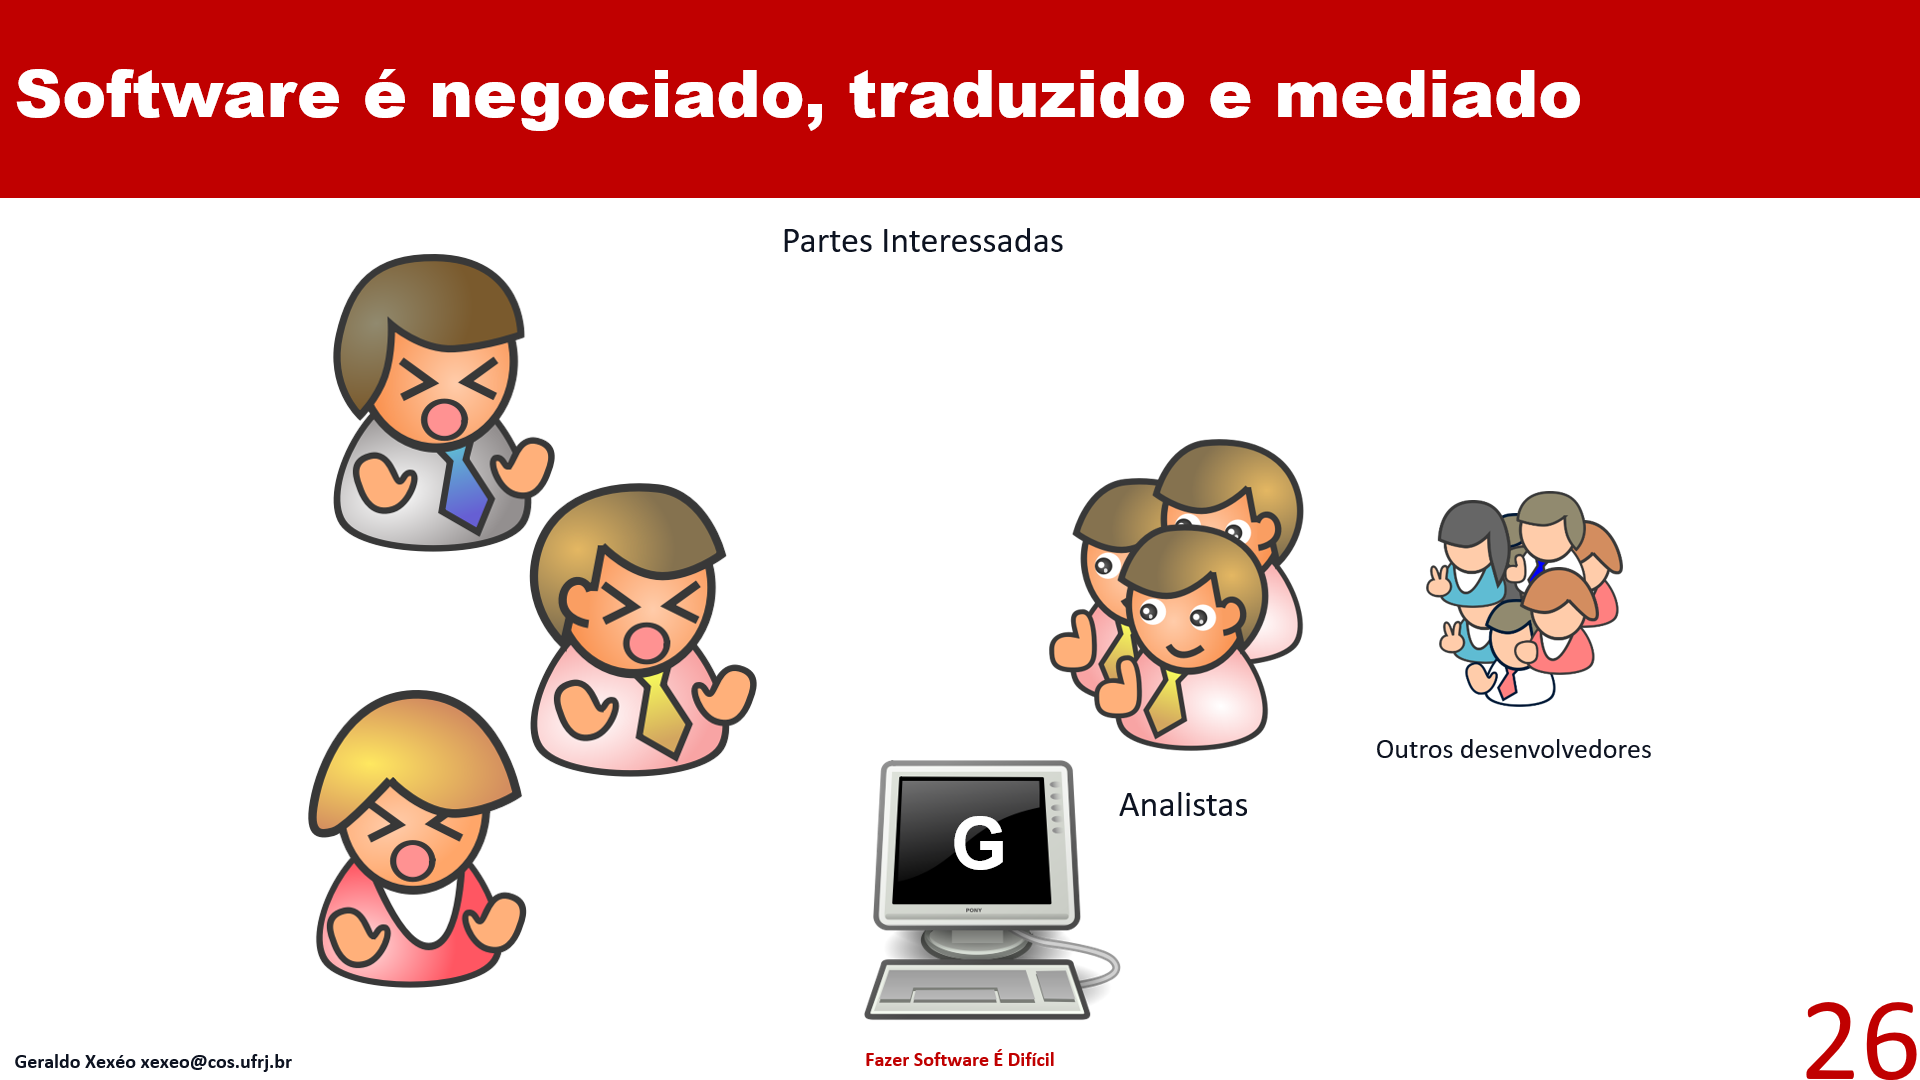
\includegraphics[width=0.4\linewidth,frame]{imagens/passo2}}
    \caption{Dois passos de uma animação que mostra como um software pode dar errado.}
    \label{fig:passos}
\end{figure}

Já a Figura \ref{fig:beamer} mostra como o beamer gera uma animação, a partir do código exemplo da Listagem \ref{list:beamer}. Nesse caso, foi usada a opção de mostrar e apagar os itens, já que se apresentava uma interface de programa e seria contraproducente manter muita informação na tela.

\begin{figure}[hbt]
    \centering
    \subfloat{
        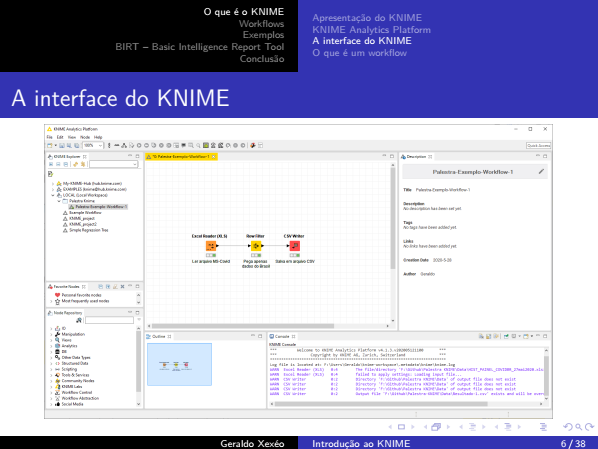
\includegraphics[width=0.4\linewidth,frame]{imagens/beamer0}}
    \subfloat{
    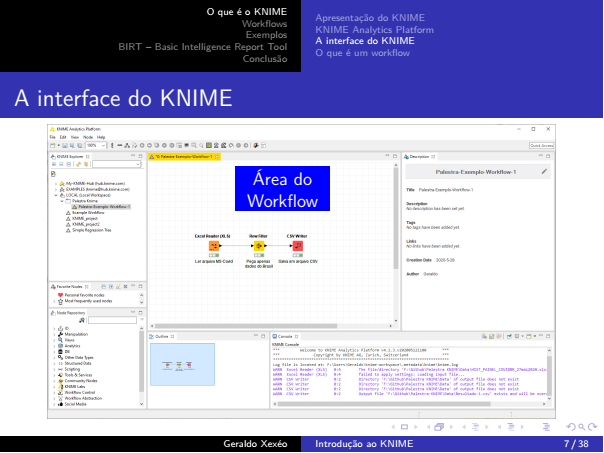
\includegraphics[width=0.4\linewidth,frame]{imagens/beamer1}}
\\
    \subfloat{
    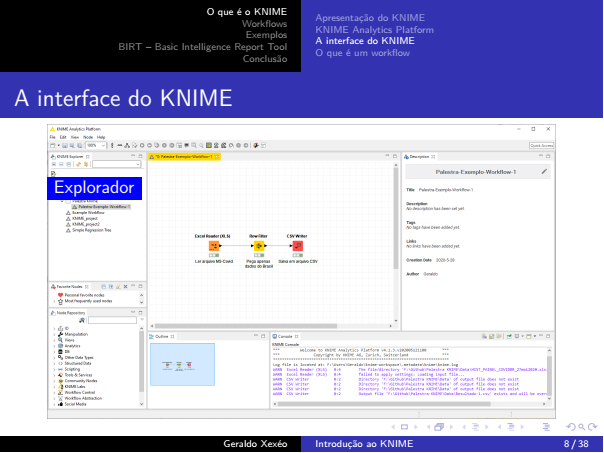
\includegraphics[width=0.4\linewidth,frame]{imagens/beamer2}}
    \subfloat{
    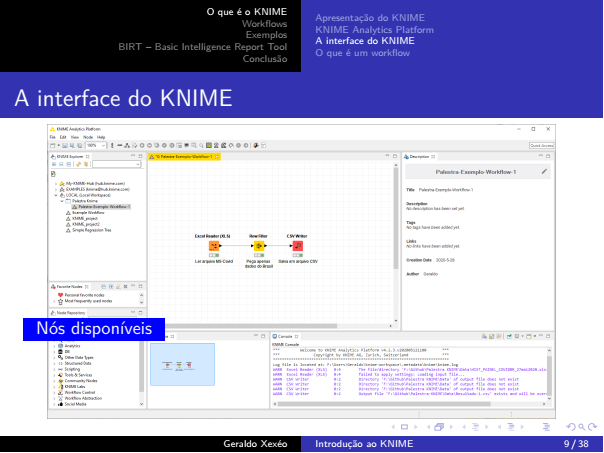
\includegraphics[width=0.4\linewidth,frame]{imagens/beamer3}}

    \caption{Quatro passos de uma animação criada pelo \texttt{beamer}. Ele gera um slide em PDF para cada passo, porém mantém apenas um item na agenda do cabeçalho e nos \textit{bookmarks} do arquivo \texttt{.pdf}.}
    \label{fig:beamer}
\end{figure}

\begin{lstlisting}[language=TeX,caption={Código \LaTeX\ para gerar os slides da Figura \ref{fig:beamer}},label={list:beamer}]
\subsection{A interface do KNIME}
\begin{frame}{A interface do KNIME}
    %   \TPGrid[40mm,20mm]{10}{5}
    \only<1->{
        \centering
        \includegraphics[width=\linewidth]{Images/Interface1}
    }
    \setlength{\TPHorizModule}{\textwidth}
    \setlength{\TPVertModule}{\textheight}
    \only<2>{
        \begin{textblock*}{20mm}(60mm,40mm)\color{white}
            Área do Workflow
    \end{textblock*}}
    \only<3>{
        \begin{textblock*}{20mm}(20mm,40mm)
            \color{white} Explorador
    \end{textblock*}}
    \only<4>{
        \begin{textblock*}{30mm}(20mm,70mm)
            \color{white}Nós disponíveis
    \end{textblock*}}
\end{frame}
\end{lstlisting}